\def\duedate{11/12/22}
\def\HWnum{9}
% Document setup
\documentclass[12pt]{article}
\usepackage[margin=1in]{geometry}
\usepackage{fancyhdr}
\usepackage{lastpage}

\pagestyle{fancy}
\lhead{Richard Whitehill}
\chead{MATH 757 -- HW \HWnum}
\rhead{\duedate}
\cfoot{\thepage \hspace{1pt} of \pageref{LastPage}}

% Encoding
\usepackage[utf8]{inputenc}
\usepackage[T1]{fontenc}

% Math/Physics Packages
\usepackage{amsmath}
\usepackage{amssymb}
\usepackage{mathtools}
\usepackage[arrowdel]{physics}
\usepackage{siunitx}

\AtBeginDocument{\RenewCommandCopy\qty\SI}

% Reference Style
\usepackage{hyperref}
\hypersetup{
    colorlinks=true,
    linkcolor=blue,
    filecolor=magenta,
    urlcolor=cyan,
    citecolor=green
}

\newcommand{\eref}[1]{Eq.~(\ref{eq:#1})}
\newcommand{\erefs}[2]{Eqs.~(\ref{eq:#1})--(\ref{eq:#2})}

\newcommand{\fref}[1]{Fig.~\ref{fig:#1}}
\newcommand{\frefs}[2]{Figs.~\ref{fig:#1}--\ref{fig:#2}}

\newcommand{\tref}[1]{Table~\ref{tab:#1}}
\newcommand{\trefs}[2]{Tables~\ref{tab:#1}-\ref{tab:#2}}

% Figures and Tables 
\usepackage{graphicx}
\usepackage{float}

\newcommand{\bef}{\begin{figure}[h!]\begin{center}}
\newcommand{\eef}{\end{center}\end{figure}}

\newcommand{\bet}{\begin{table}[h!]\begin{center}}
\newcommand{\eet}{\end{center}\end{table}}

% tikz
\usepackage{tikz}
\usetikzlibrary{calc}
\usetikzlibrary{decorations.pathmorphing}
\usetikzlibrary{decorations.markings}
\usetikzlibrary{arrows.meta}
\usetikzlibrary{positioning}

% tcolorbox
\usepackage[most]{tcolorbox}
\usepackage{xcolor}
\usepackage{xifthen}
\usepackage{parskip}

\newcommand*{\eqbox}{\tcboxmath[
    enhanced,
    colback=black!10!white,
    colframe=black,
    sharp corners,
    size=fbox,
    boxsep=8pt,
    boxrule=1pt
]}

% Miscellaneous Definitions/Settings
\newcommand{\prob}[2]{\textbf{#1)} #2}
\newcommand{\reals}{\mathbb{R}}
\newcommand{\integers}{\mathbb{Z}}
\newcommand{\naturals}{\mathbb{N}}
\newcommand{\rationals}{\mathbb{Q}}
\newcommand{\complexs}{\mathbb{C}}

\setlength{\parskip}{\baselineskip}
\setlength{\parindent}{0pt}
\setlength{\headheight}{14.49998pt}
\addtolength{\topmargin}{-2.49998pt}







\begin{document}
    
\prob{Lecture 16 - 2}{
Use the recurrence relations
\begin{eqnarray}
    \label{eq:recurrence-7}
    (2n+1)xP_{n}(x) = (n+1)P_{n+1}(x) + nP_{n-1}(x) 
\end{eqnarray}
and
\begin{eqnarray}
    \label{eq:recurrence-8}
    P_{n+1}'(x) + P_{n-1}'(x) = 2xP_{n}'(x) + P_{n}(x) 
\end{eqnarray}
to show that 
\begin{eqnarray}
    \label{eq:recurrence-9}
    P_{n+1}'(x) - P_{n-1}'(x) = (2n+1)P_{n}(x) 
.\end{eqnarray}
}

Let us differentiate \eref{recurrence-7}:
\begin{eqnarray}
    \label{eq:diff-recurrence-7}
    (2n+1)P_{n}(x) + (2n+1)xP_{n}'(x) = (n+1)P_{n+1}'(x) + nP_{n-1}'(x)
.\end{eqnarray}
From \eref{recurrence-8}, we see that
\begin{eqnarray}
    \label{eq:rewrite-recurrence-8}
    2xP_{n}'(x) = P_{n+1}'(x) + P_{n-1}'(x) - P_{n}(x) 
.\end{eqnarray}
Hence, \eref{diff-recurrence-7} becomess
\begin{gather}
\label{eq:final-recurrence}
    2(2n+1)P_{n}(x) + (2n+1)[P_{n+1}'(x) + P_{n-1}'(x) - P_{n}(x)] = 2(n+1)P_{n+1}'(x) + 2nP_{n-1}'(x) \notag \\
    [(2n+1) - (2n+2)]P_{n+1}'(x) + [(2n+1) - 2n]P_{n-1}'(x) = -[(4n+2) - (2n+1)]P_{n}(x) \notag \\
    -P_{n+1}'(x) + P_{n-1}'(x) = -(2n + 1)P_{n}(x) \notag \\
    \eqbox{P_{n+1}'(x) - P_{n-1}'(x) = (2n+1)P_{n}(x)}
.\end{gather}




\prob{Lecture 16 - 3}{
Show that
\begin{eqnarray}
    \label{eq:gen-func}
    g(x,t) = \frac{1}{\sqrt{1 - 2xt + t^2}} 
\end{eqnarray}
satisfies the differential equation
\begin{eqnarray}
    \label{eq:diff-gen-func}
    \pdv{x} \Big[ (1-x^2)\pdv{x} g(x,t) \Big] + t \pdv[2]{t} \Big[ tg(x,t) \Big] = 0
.\end{eqnarray}
}

For this problem, we simply take derivatives:
\begin{align}
    \label{eq:derivs-1}
    \pdv{g}{x} &= \frac{t}{(1 - 2xt + t^2)^{3/2}} \\
    %
    \label{eq:derivs-2}
    \pdv{x}(1-x^2)\pdv{g}{x} &= -\frac{t(2t^2x - tx^2 - 3t + 2x)}{(1 - 2xt + t^2)^{5/2}} \\
    %
    t \pdv[2]{(tg)}{t} &= t\pdv{t} \Bigg[ \frac{1 - xt}{(1 - 2xt + t^2)^{3/2}} \Bigg] \notag \\
    \label{eq:derivs-3}
                     &= \frac{t(2t^2x - tx^2 - 3t + 2x)}{(1 - 2xt + t^2)^{5/2}}
.\end{align}
Clearly, the expressions in \eref{derivs-2} and \eref{derivs-3} match up to a minus sign, so $g(x,t)$ satisfies the differential equation given by \eref{diff-gen-func}.


\prob{Lecture 17 - 1}{
Check that 
\begin{eqnarray}
    \label{eq:ex1-res}
    \langle Au, v \rangle = \langle u, Av \rangle \iff p(x)\big[ u'v - uv' \big]\big|_{a}^{b} = 0
.\end{eqnarray}
}

The inner product on $L_{2,w}(a,b)$ (where $w(x) > 0$ for all $x \in (a,b)$)
\begin{eqnarray}
    \label{eq:inner-product}
    \langle u,v \rangle = \int_{a}^{b} w(x) u(x) v(x) \dd{x}
,\end{eqnarray}
and the operator $A$ is defined such that
\begin{eqnarray}
    \label{eq:operator-A}
    Au = -\frac{1}{w(x)}\Big[ \partial_{x} \big( p(x) \partial_{x} u \big) + q(x) u \Big] 
,\end{eqnarray}
where $p(x) > 0$ and $q(x)$ is a real-valued function on $(a,b)$.

Assuming that $\langle Au,v \rangle = \langle u,Av \rangle$ holds, then
\begin{eqnarray}
    \label{eq:forward-direc}
    \int_{a}^{b} \Big[ \partial_{x} \big( p(x)\partial_{x}u(x) \big) + q(x)u(x) \Big] v(x) \dd{x} = \int_{a}^{b} u(x) \Big[ \partial_{x} \big( p(x)\partial_{x}v(x) \big) + q(x)v(x) \Big] \dd{x}
,\end{eqnarray}
where $w(x)$ vanishes here since it is strictly positive.
Simplifying, we find
\begin{eqnarray}
    \label{eq:simplify-forward-direc}
    \int_{a}^{b} \Big[ p'u'v + pu''v - up'v' - upv'' \Big] \dd{x} = 0
.\end{eqnarray}
We can now integrate by parts on the terms containing derivatives of $p(x)$ such that
\begin{eqnarray}
    \label{eq:int-by-parts}
    pu'v|_{a}^{b} - upv'|_{a}^{b} + \int_{a}^{b} \big[ p\partial_{x}(u'v) + pu''v - p\partial_{x}(uv') - upv'' \big] \dd{x} = 0
.\end{eqnarray}
Upon taking derivatives and simplifying, we realize that the integrand in the second term is identically zero, leaving us with
\begin{eqnarray}
    \label{eq:forward-res}
    p(x) \big[ u'(x)v(x) - u(x)v'(x) \big]\big|_{a}^{b} = 0
.\end{eqnarray}

Now we assume that \eref{forward-res} holds true.
Thus,
\begin{align}
    \label{eq:backward-direc}
    \langle Au,v \rangle &= \int_{a}^{b} \Big[ \partial_{x} \big( p(x)\partial_{x}u(x) \big) + q(x)u(x) \Big] v(x) \dd{x} \notag \\
                         &= \int_{a}^{b} \big[ p'u'v + pu''v + qvu \big] \dd{x} \notag \\
                         %
                         &= pu'v|_{a}^{b} + \int_{a}^{b} \big[ -pu''v - pu'v' + pu''v + qvu \big] \dd{x} \\
                         &= pu'v|_{a}^{b} - puv'|_{a}^{b} + \int_{a}^{b} \big[ p'v' + pv'' + qvu \big] \dd{x} \notag \\
                         &= \langle u,Av \rangle
,\end{align}
which concludes the second portion of the proof, showing a necessary and sufficient condition for operator $A$ to be symmetric.

\prob{Lecture 17 - 2}{
Check that for operator $A$ given by \eref{operator-A}
\begin{eqnarray}
    \label{eq:res-17.2}
    \langle Au,u \rangle = -p(x) u' u \big|_{a}^{b} + \int_{a}^{b} [p(x)|u'(x)|^2 - q(x)|u|^2] \dd{x}
.\end{eqnarray}
}

We can steal the form of \eref{backward-direc} and substitute $v = u$, which gives us that
\begin{eqnarray}
    \label{eq:res-17.2-work}
    \eqbox{
    \langle Au,u \rangle =  p(x)u'(x)u(x) \big|_{a}^{b} - \int_{a}^{b} \big[ p(x)|u'(x)|^2 - q(x)|u(x)|^2 \big] \dd{x}
}
.\end{eqnarray}



\prob{Lecture 17 - 3}{
For all $u,v \in C^2(\overline{\Omega})$, where $\overline{\Omega} = \Omega \cup \partial \Omega$ ($\Omega$ is bounded), check the so-called Green's identities
\begin{eqnarray}
    \label{eq:Green-identity-1}
    \langle Au,v \rangle - \langle u,Av \rangle = \int_{\Omega} p \Big( u \pdv{v}{n} - v \pdv{u}{n} \Big) \dd{S}
,\end{eqnarray}
where $\partial_{n} = \hat{n} \cdot \nabla$ is the directional derivative along the direction normal to the surface of $\Omega$,
\begin{eqnarray}
    \label{eq:Green-identity-2}
    \langle Au,u \rangle = - \int_{\partial \Omega} pu\pdv{u}{n} \dd{S} + \int_{\Omega} \big[ p|\nabla u|^2 - q|u|^2 \big] \dd[3]{x}
.\end{eqnarray}
}

\begin{figure}[H]
\begin{center}
    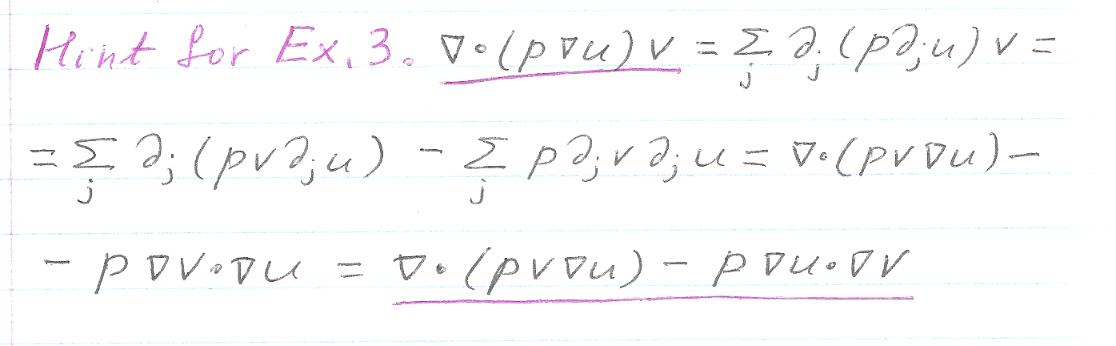
\includegraphics[width=0.7\textwidth]{hint3.png}
\end{center} 
\end{figure}

The multi-dimensional operator $A$ is defined in analogy with the one-dimensional version such that
\begin{eqnarray}
    \label{eq:operator-A-multidim}
    Au = -\frac{1}{w(x)} \Big[ \nabla \cdot (p \nabla u) + qu \Big] 
,\end{eqnarray}
and the inner product is defined in analogy with the one-dimensional version as
\begin{eqnarray}
    \label{eq:inner-product-multidim}
    \langle u,v \rangle \int_{\Omega} w(x) u(x) v(x) \dd[3]{x}
.\end{eqnarray}

Checking the first identity is quite simple then:
\begin{align}
    \label{eq:Green-identity-1-verify}
    \langle Au,v \rangle - \langle u,Av \rangle = \int_{a}^{b} \Big[ v \nabla \cdot (p \nabla u) - u \nabla \cdot (p \nabla v) \Big] \dd[3]{x}
.\end{align}


\prob{Lecture 17 - 4}{
Find eigenvectors and eigenvalues for operator $A$, defined such that $Au = - \Delta u$ (defined in Example 2) in the following cases.
}

4.1) $\mathcal{D}(A) = \{ u \in C^2(\overline{\Omega}) \,:\, u(x,0) = u(x,H) = 0,\, u_{y}(0,y) = u_{y}(L,y) = 0 \}$

4.2) $\mathcal{D}(A) = \{ u \in C^2(\overline{\Omega}) \,:\, u(0,y) = u(L,y), \, u(x,0) = u(x,H),\, u_{y}(0,y) = u_{y}(L,y), \\ \, u_{x}(x,0) = u_{x}(x,H) \}$




\end{document}
